\documentclass{beamer}
%\documentclass[handout]{beamer}

% language settings
%\usepackage{fontspec, polyglossia}
%\setdefaultlanguage{magyar}

% common packages
\usepackage{amsmath, multimedia, hyperref, color, multirow}
%\usepackage{graphicx}

% TikZ
\usepackage{tikz}
%\usetikzlibrary{arrows.meta, decorations.pathmorphing, decorations.pathreplacing, shapes.geometric,mindmap}
%\usetikzlibrary{shapes.geometric,fadings,bayesnet}

% beamer styles
\mode<presentation>{
\usetheme{Warsaw}
%\usetheme{Antibes}
\usecolortheme{beaver}
%\usecolortheme{seahorse}
%\usefonttheme{structureitalicserif}
\setbeamercovered{transparent}
}
\setbeamertemplate{blocks}[rounded][shadow=true]
\AtBeginSubsection[]{
  \begin{frame}<beamer>{Contents}
    \tableofcontents[currentsection,currentsubsection]
  \end{frame}
}
%\useoutertheme[]{tree}

% title, etc
\title{Somatic Mutations in the Human Brain from NGS data}
%\subtitle{A subtitle may be shorter and more technical}
\author{Attila Gulyas-Kovacs}
\date{Chess Lab}

\begin{document}

\maketitle

\begin{frame}{Genetics of psychiatric disorders}
\begin{itemize}
\item germline variants
\item \textit{de novo} variants
\item<2-> gene-gene and gene-environment interactions  
\item<3-> somatic variants
\begin{itemize}
%\item<3-> \alert{our hypothesis: psychiatric disorders; schizophrenia}
\item cancer, aging
\item V(D)J recombination
\item dysplasias: hemimegencephaly, lissencephaly, pediatric epilepsy 
\item<4-> \alert{psychiatric disorders?}\\
Brain Somatic Mosaicism Network (BSMN)
\end{itemize}
\end{itemize}
\end{frame}

\begin{frame}{Patterns of somatic mosaicism}
\includegraphics[width=1.0\textwidth]{figures/from-others/lodato2015science-fig3ab.png}
\end{frame}

\begin{frame}{Embryonic development}
%gastrulation video
%https://www.youtube.com/watch?v=3AOoikTEfeo
%neurulation video
%https://www.youtube.com/watch?v=lGLexQR9xGs
\includegraphics[height=0.8\textheight]{figures/from-others/HumanEmbryogenesis.png}
\end{frame}

\begin{frame}{Neocortical development}
\includegraphics[height=0.8\textheight]{figures/from-others/doi_10_1016-j_cell_2011_06_030-fig4b-neocortical-development.jpg}
\end{frame}

\begin{frame}{Mutation rate}
\includegraphics[width=0.8\columnwidth]{figures/from-others/lynch-evolution-of-mutation-rate-fig3.jpg}
\end{frame}

\begin{frame}{Sequencing approaches to detect somatic variants}
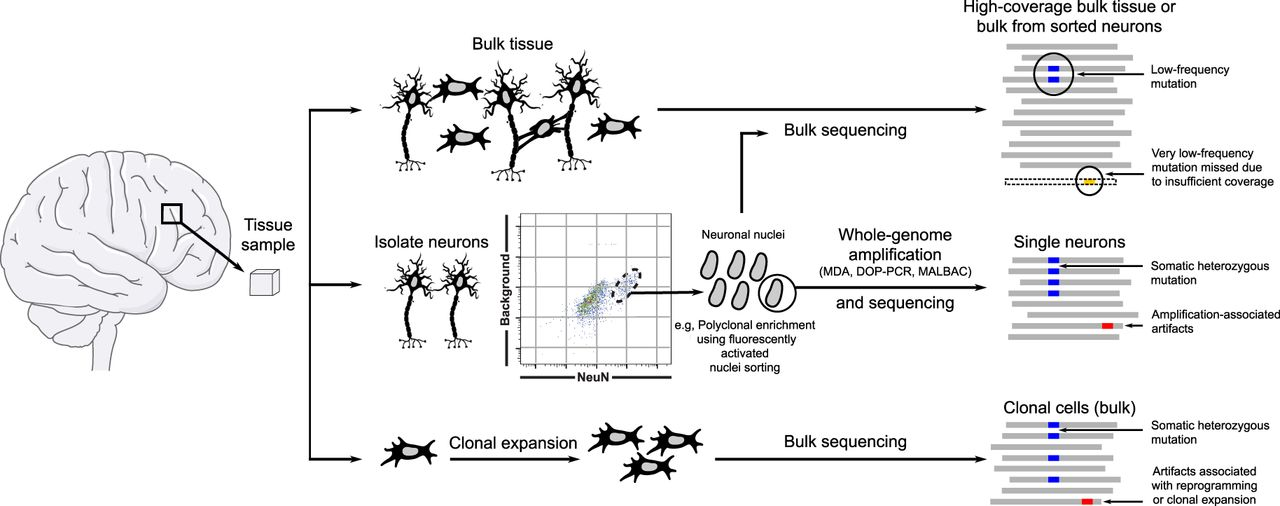
\includegraphics[width=1.0\textwidth]{figures/from-others/bsm-science-fig2.jpg}
\end{frame}

\begin{frame}{Discordance between variant callers}

\begin{columns}[t]
\begin{column}{0.5\textwidth}

\includegraphics[width=1.0\columnwidth]{figures/2018-11-06-number-of-calls/snvs-cs-1.pdf}
\end{column}

\begin{column}{0.6\textwidth}

\includegraphics<2>[width=1.0\columnwidth]{figures/2018-04-08-call-set-concordance/venn-common-sample-wgs-snvs-1.pdf}
\end{column}
\end{columns}
\end{frame}

\begin{frame}{Heuristic filtering and combination of call sets}
\tiny
\setlength{\tabcolsep}{3pt}
\begin{tabular}{l|llllllll|}
\footnotesize &
\multicolumn{8}{c}{\footnotesize \texttt{TNseq.Mutect2.vcf}} \\
\hline
 & \#CHROM & POS & ID & REF & ALT & QUAL & FILTER & INFO \\
\textcolor{cyan}{\(c\)} &
\textcolor{cyan}{1} &
\textcolor{cyan}{50003788} &
\textcolor{cyan}{0} &
\textcolor{cyan}{A} &
\textcolor{cyan}{G} &
\textcolor{cyan}{0} &
\textcolor{cyan}{t\_lod\_fstar} &
\textcolor{cyan}{...;NLOD=30.4;TLOD=4.62} \\
\textcolor{cyan!50!brown}{\(d\)} &
\textcolor{cyan!50!brown}{1} &
\textcolor{cyan!50!brown}{50005034} &
\textcolor{cyan!50!brown}{0} &
\textcolor{cyan!50!brown}{G} &
\textcolor{cyan!50!brown}{T} &
\textcolor{cyan!50!brown}{0} &
\textcolor{cyan!50!brown}{t\_lod\_fstar} &
\textcolor{cyan!50!brown}{...;NLOD=33.27;TLOD=4.51} \\
\textcolor{cyan!50!brown}{\(e\)} &
\textcolor{cyan!50!brown}{1} &
\textcolor{cyan!50!brown}{50007349} &
\textcolor{cyan!50!brown}{0} &
\textcolor{cyan!50!brown}{C} &
\textcolor{cyan!50!brown}{T} &
\textcolor{cyan!50!brown}{0} &
\textcolor{cyan!50!brown}{PASS} &
\textcolor{cyan!50!brown}{...;NLOD=23.43;TLOD=10.97} \\
\textcolor{cyan!50!brown}{\(f\)} &
\textcolor{cyan}{1} &
\textcolor{cyan}{50008565} &
\textcolor{cyan}{0} &
\textcolor{cyan}{C} &
\textcolor{cyan}{A} &
\textcolor{cyan}{0} &
\textcolor{cyan}{PASS} &
\textcolor{cyan}{...;NLOD=7.69;TLOD=8.26} \\
\hline
% \vdots & \vdots & \vdots & \vdots & \vdots & \vdots & \vdots & \vdots & \vdots & \vdots & \vdots \\
\end{tabular}
\tiny
\\[1em]
\begin{tabular}{l|llllllll|}
\footnotesize &
\multicolumn{8}{c}{\footnotesize \texttt{strelka2Somatic.vcf}} \\
\hline
 & \#CHROM & POS & ID & REF & ALT & QUAL & FILTER & INFO \\
\textcolor{brown}{\(a\)} &
\textcolor{brown}{1} &
\textcolor{brown}{50003323} &
\textcolor{brown}{0} &
\textcolor{brown}{A} &
\textcolor{brown}{G} &
\textcolor{brown}{0} &
\textcolor{brown}{LowEVS} &
\textcolor{brown}{...;DP=274;MQ=59.86;...;SomaticEVS=0} \\
\textcolor{brown}{\(b\)} &
\textcolor{brown}{1} &
\textcolor{brown}{50003455} &
\textcolor{brown}{0} &
\textcolor{brown}{C} &
\textcolor{brown}{T} &
\textcolor{brown}{0} &
\textcolor{brown}{LowEVS} &
\textcolor{brown}{...;DP=226;MQ=59.9;...;SomaticEVS=0.65} \\
\textcolor{brown}{\(d\)} &
\textcolor{cyan!50!brown}{1} &
\textcolor{cyan!50!brown}{50005034} &
\textcolor{cyan!50!brown}{0} &
\textcolor{cyan!50!brown}{G} &
\textcolor{cyan!50!brown}{T} &
\textcolor{cyan!50!brown}{0} &
\textcolor{cyan!50!brown}{PASS} &
\textcolor{cyan!50!brown}{...;DP=278;MQ=59.95;...;SomaticEVS=9.04} \\
\textcolor{brown}{\(e\)} &
\textcolor{cyan!50!brown}{1} &
\textcolor{cyan!50!brown}{50007349} &
\textcolor{cyan!50!brown}{0} &
\textcolor{cyan!50!brown}{C} &
\textcolor{cyan!50!brown}{T} &
\textcolor{cyan!50!brown}{0} &
\textcolor{cyan!50!brown}{LowEVS} &
\textcolor{cyan!50!brown}{...;DP=192;MQ=59.88;...;SomaticEVS=4.19} \\
\hline
% \vdots & \vdots & \vdots & \vdots & \vdots & \vdots & \vdots & \vdots & \vdots & \vdots & \vdots \\
\end{tabular}
% ##INFO=<ID=SomaticEVS,Number=1,Type=Float,Description="Somatic Empirical
% Variant Score (EVS) expressing the phred-scaled probability of thecall being
% a false positive observation.">
\normalsize


\includegraphics[height=0.6\textheight]{figures/Tnseq-4-strelka2Somatic-4-venn.png}
\end{frame}

\begin{frame}{Discordance between research groups}
\includegraphics[height=0.7\columnwidth]{figures/from-others/bsmn-cs-callset-concordance.png}
\end{frame}

\begin{frame}
How to find the best calling approach?
\begin{itemize}
\item consortium
\begin{enumerate}
\item real data set
\item heuristic filtering and combination of call sets
\item validate some calls with targeted resequencing 
\item refine heuristics
\item ...  
\end{enumerate}
\item<2> our group
\begin{enumerate}
\item benchmark data set with known variants
\item select annotations in call sets
\item input to machine learning\footnote{VariantMetaCaller}
\item validate all calls
\item re-select annotations 
\item ...
\end{enumerate}
\end{itemize}
\end{frame}

\end{document}


\begin{columns}[t]
\begin{column}{0.5\textwidth}

\end{column}

\begin{column}{0.5\textwidth}

\end{column}
\end{columns}
